%%%%%%%%%%%%%%%%%%%%%%%%%%%%%%%%%%%%%%%%%%%%%%%%%%%%%%%%%%%%%%%%%%%%%%%%%%%%%%%%%%%%
%Do not alter this block of commands.  If you're proficient at LaTeX, you may include additional packages, create macros, etc. immediately below this block of commands, but make sure to NOT alter the header, margin, and comment settings here.
\documentclass[12pt]{article}
 \usepackage[margin=1in]{geometry}
 \usepackage[utf8]{inputenc}
\usepackage[spanish]{babel}
\usepackage{amsmath,amsthm,amssymb,amsfonts, enumitem, fancyhdr, color, comment, graphicx, environ}
\pagestyle{fancy}
\setlength{\headheight}{65pt}
\newenvironment{problem}[2][Problem]{\begin{trivlist}
\item[\hskip \labelsep {\bfseries #1}\hskip \labelsep {\bfseries #2.}]}{\end{trivlist}}
\newenvironment{sol}
    {\emph{Solution:}
    }
    {
    \qed
    }
\specialcomment{com}{ \color{blue} \textbf{Comment:} }{\color{black}} %for instructor comments while grading
\NewEnviron{probscore}{\marginpar{ \color{blue} \tiny Problem Score: \BODY \color{black} }}
%%%%%%%%%%%%%%%%%%%%%%%%%%%%%%%%%%%%%%%%%%%%%%%%%%%%%%%%%%%%%%%%%%%%%%%%%%%%%%%%%





%%%%%%%%%%%%%%%%%%%%%%%%%%%%%%%%%%%%%%%%%%%%%
%Fill in the appropriate information below
\lhead{Cristóbal Meneses}  %replace with your name
\rhead{Tópicos de Microeconometría  \\ Tarea 1} %replace XYZ with the homework course number, semester (e.g. ``Spring 2019"), and assignment number.
%%%%%%%%%%%%%%%%%%%%%%%%%%%%%%%%%%%%%%%%%%%%%


%%%%%%%%%%%%%%%%%%%%%%%%%%%%%%%%%%%%%%
%Do not alter this block.
\begin{document}
%%%%%%%%%%%%%%%%%%%%%%%%%%%%%%%%%%%%%%


%Solutions to problems go below.  Please follow the guidelines from https://www.overleaf.com/read/sfbcjxcgsnsk/


%Copy the following block of text for each problem in the assignment.
\begin{problem}{A.1}
En los datos de panel del programa PROGRESA, podemos observar que existen observaciones para 28210 niños en dos periodos. Estos datos estan fuertemente balanceados.
\end{problem}



%Copy the following block of text for each problem in the assignment.
\begin{problem}{A.2}
A través de un promedio de la variable tcomm, la cual es equivalente a una probabilidad, observamos que 60,5636\% de los niños en la muestra esta en un pueblo elegido para el tratamiento. Este porcentaje es constante en el tiempo.
\end{problem}




%Copy the following block of text for each problem in the assignment.
\begin{problem}{A.3}
Ya que el programa PROGRESA esta orientado a localidades y no directamente a individuos, hay factores que no pudieron ser controlados por los investigadores. Uno de estos es que en pueblos con individuos pobres, individuos no-pobres pudieron acceder al programa. En efecto, si hubiesen sido aplicado perfectamente el problema, la correlacion entre ser tratado y ser pobre hubiese sido de 1 (lo que no es el caso, con una correlacion de +0,033). De los 28210 niños observados, 5616 son niños pobres no en pueblos de control y 7112 son niños no-pobres en pueblos tratados, quedando el resto o en la categoria de niños pobres tratados o en niños no-pobres en control.
\end{problem}



%Copy the following block of text for each problem in the assignment.
\begin{problem}{A.4}
De los 28210 niños tratados, 18581(65,87\%) son pobres y 9629 (34,13\%) son no-pobres. Esta proporción se mantiene cuando vemos la distribución de pobreza en las comunas tratadas. De los 17085 niños en un pueblo tratado, 11469(67,13\%) son pobres y 5616(32,87\%) son no-pobres. Por esto, podemos ver que 7112 niños pobres no eran elegibles para el programa por su ubicación geográfica y quedaron en el grupo de control.
\end{problem}



%Copy the following block of text for each problem in the assignment.
\begin{problem}{A.5}
Vemos en una comparacion grafica de la clasificación de pobreza de pobres y no-pobres. Existe una calra diferencia grafica, que refleja que en caso de ser pobre se tiene un puntaje promedio de riqueza de 621, mas de doscientos puntos debajo del promedio de no-pobres de 832 \\

\centering
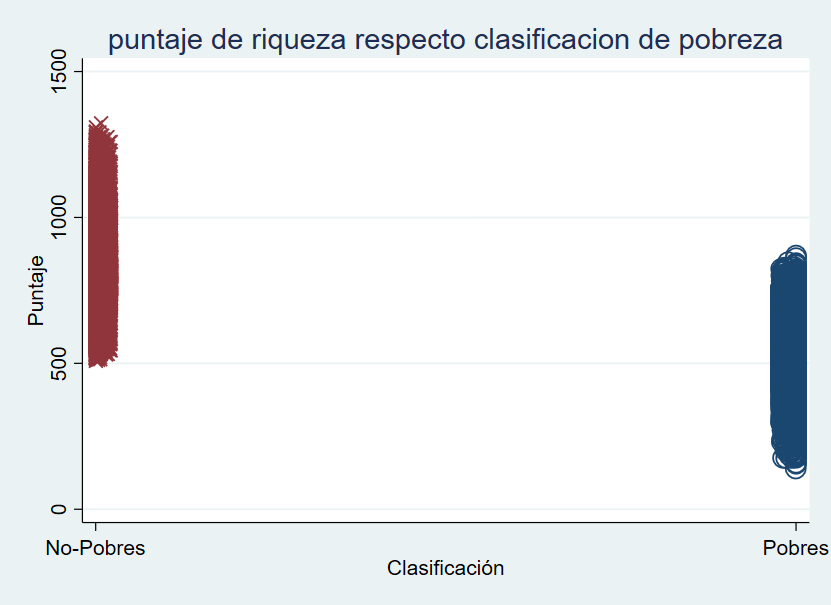
\includegraphics[width=11.634cm, height=8.47cm]{pobreza.png}

\end{problem}




%Copy the following block of text for each problem in the assignment.
\begin{problem}{B.1}
El estimador es de $\hat{\beta}=$0.0476. Esto significaría que
$$enrolled_i=0.6508+0.0476*tcomm_i$$
\end{problem}




%Copy the following block of text for each problem in the assignment.
\begin{problem}{B.2}
Para que la regresión anterior sea valida necesitariamos un nivel de inconfundibilidad no condicionada tal que que tu localidad sea seleccionada para el experimento ocurra de forma independiente a cualquier otra variable.
\end{problem}



%Copy the following block of text for each problem in the assignment.
\begin{problem}{B.3}
Esta condición no se cumple debido a que se seleccionaron localidades con mayor indice de pobreza, como se muestra en la respuesta a la pregunta A.4. Como sabemos que localidades con mayor pobreza fueron elegidas para el experimento, el efecto marginal de ser elegido no puede ser estimado inmediatamente con una diferencia de medias pues hay mas variables que afectan a la selección.
\end{problem}




%Copy the following block of text for each problem in the assignment.
\begin{problem}{D.1}
Generamos un puntaje de propensidad a partir de las variables individuales de los niños $age$, $female$ y $pobre$. Estos puntajes se dividen en 4 bloques con igual promedio para asegurar las condiciones de unconfoundedness.
\end{problem}

%Copy the following block of text for each problem in the assignment.
\begin{problem}{D.2}\\
Se observan los 4 bloques equivalentes. Con estos, podemos decir que se cumple la condicion de overlap requerida para la de unconfoundedness.\\
\centering
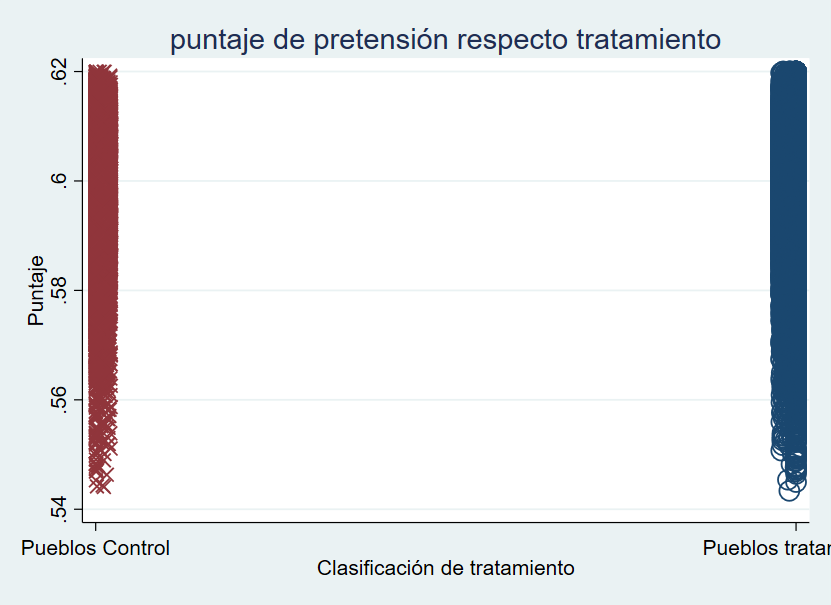
\includegraphics[width=11.634cm,height=8.47cm]{pretencion.png}

\end{problem}



%Copy the following block of text for each problem in the assignment.
\begin{problem}{D.3}
Con un emparejamiento del tipo vecino mas cercano se observa un ATT de 0.067585232 con una desciación estándard de 0.023370607, mientras que ocupando un emparejamiento de grupos (cluster) es de 0.014869138 con una desviación de 0.003937542. En ambos casos el ATT es positivo y estadisticamente significativo, aunque tienen una diferencia de 0.05271609 que, si interpretamos como diferencia de efecto marginal de tratados, es bastante grande.
\end{problem}






























%%%%%%%%%%%%%%%%%%%%%%%%%%%%%%%%%%%%%%%%
%Do not alter anything below this line.
\end{document}
